\section{Introduction}

Single-cell transcriptomics provides a high-resolution view of cellular heterogeneity, enabling the study of diverse cell states within complex tissues. However, these measurements are inherently sparse and noisy~\citep{luecken2019current}, making it difficult to reliably recover the underlying biological states. A common approach to address this challenge is to aggregate similar cells into \emph{metacells}~\citep{metacell}, which provide denoised gene expression profiles that better reflect true cellular states. This relies on the assumption that variation within a group of similar cells is largely driven by noise, while shared patterns correspond to meaningful biological structure. Cell--cell affinity---a measure of pairwise similarity that guides which cells are grouped together---is central to this process and can in principle be derived from various biological sources.

Current metacell methods define this affinity based solely on gene expression and group cells that are close in this space. In multi-batch settings, batch effects distort gene expression, making similarity relationships reliable mainly within individual datasets. As a result, existing metacell methods~\citep{metacell, seacells, metacell2} form aggregations within individual batches and fail to generalize across them, even when underlying cell states are shared. This is particularly limiting for rare cell populations, where a single batch may not contain enough samples to recover stable cell states. Beyond transcriptomics, spatial organization shapes cellular programs through local interactions~\citep{nichenet, cellchat, mecell}, yet existing methods ignore this signal entirely.

We introduce \textbf{scProto}, a framework that learns metacells by preserving affinity-defined relationships while remaining faithful to gene expression data (Figure~\ref{fig:overview}). Given one or more affinity graphs, scProto encodes cells into a latent space and learns a set of shared prototypes representing metacells. Cells are probabilistically assigned to prototypes, and similarity between cells is defined through these assignments and aligned with the input affinity. This encourages highly connected cells to map to the same prototypes, preserving community structure of the affinity graph. Because the affinity is a plug-in component, the same model can preserve any biologically meaningful pairwise signal---whether transcriptomic neighborhood structure, spatial microenvironmental context, or any other relationship between cells---without architectural changes. At the same time, a reconstruction objective ensures that the learned representations capture meaningful gene expression patterns.

\begin{figure*}[t]
\centering
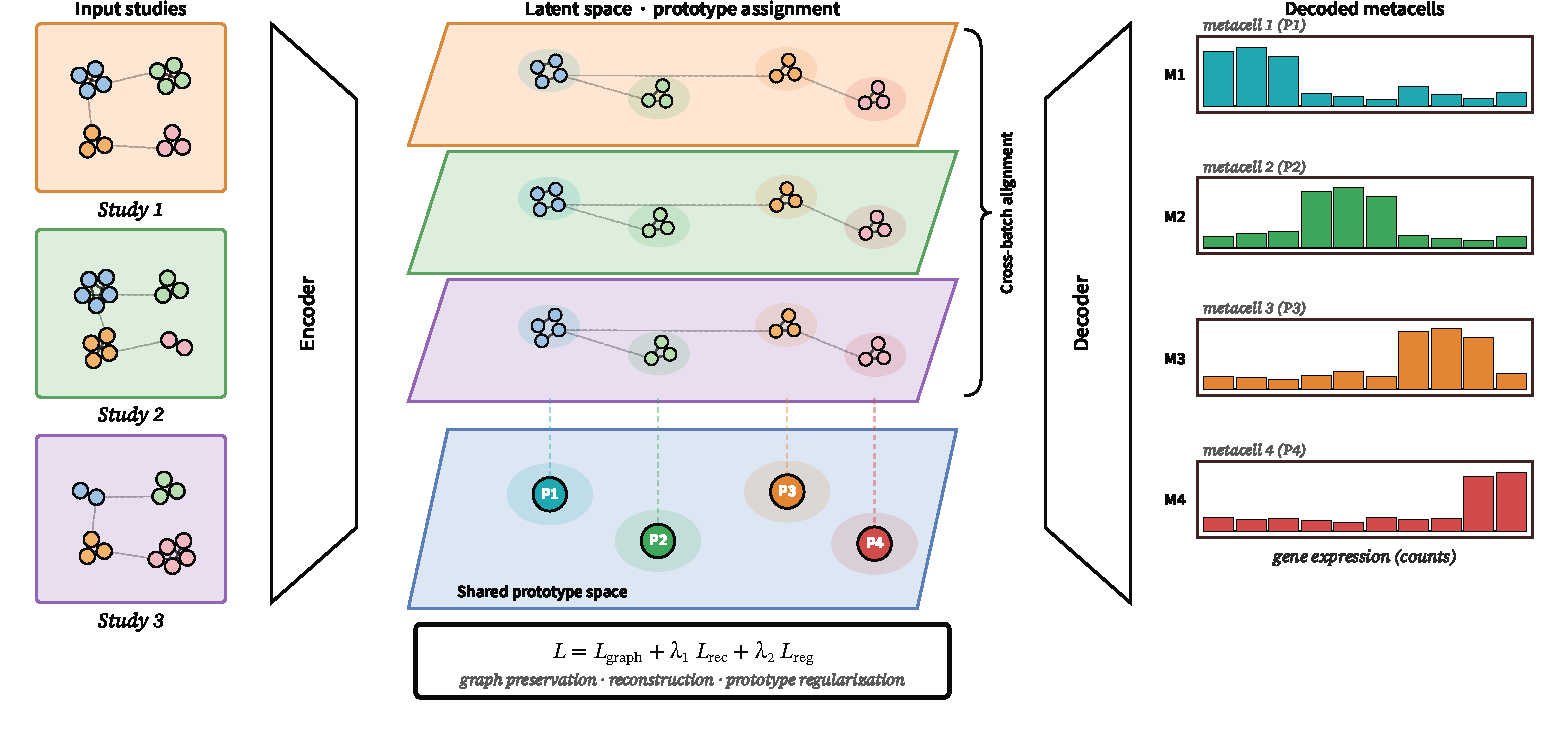
\includegraphics[width=\textwidth]{figures/scproto.pdf}
\caption{
Overview of scProto. Cells from multiple batches are encoded into a shared latent space and softly assigned to learnable prototypes (metacells). A community-preserving objective aligns prototype assignments with the input affinity graph; a reconstruction objective enables cross-batch alignment via a batch-conditional decoder.
}
\label{fig:overview}
\end{figure*}

We evaluate scProto on four datasets spanning single-cell and spatial transcriptomics. Our results show that scProto forms metacells that integrate cells across batches while preserving within-batch structure, achieving high batch mixing without sacrificing modularity and cell-type purity. This leads to improved representation of rare cell populations, where cross-batch aggregation increases effective sample size and yields more stable metacells. The flexibility of the affinity framework extends naturally to spatial settings: by defining cell--cell affinity from spatial information, scProto captures microenvironmental structure more effectively than transcriptomics-only approaches, identifying metacells that reflect both cell identity and niche-specific variation.

Our contributions are as follows:
\begin{itemize}
    \item We introduce a prototype-based framework that learns cross-batch metacells by jointly preserving affinity-defined community structure and maintaining fidelity to gene expression, with a training objective that encourages compact, distinct, and well-used prototypes.

    \item We demonstrate that combining reconstruction with affinity guidance improves cross-batch aggregation, enhances representation of rare cell populations, and enables effective integration of spatial context.
\end{itemize}